\chapter{Límite. Continuidad de una función} \label{c:limcont}


%% >>> 1
\section{Límite de una variable. Variable infinitamente grande}

\begin{definition} \index{límite!variable}
  Un número constante $a$ es el \emph{límite} de una variable $x$, si para cualquier número positivo pre-asignado $\epsilon$, arbitrariamente pequeño, es posible indicar un valor de la variable $x$ tal que todo los valores subsecuentes satisfacen la desigualdad $|x - a| < \epsilon$.
  Se dice que $x$ tiende al límite $a$: $x \to a$ o $\lim x = a$.
\end{definition}

Una interpretación geométrica del límite se puede apreciar en la figura \ref{c:limcont:vlimdef}.

\begin{figure}
  \centering

  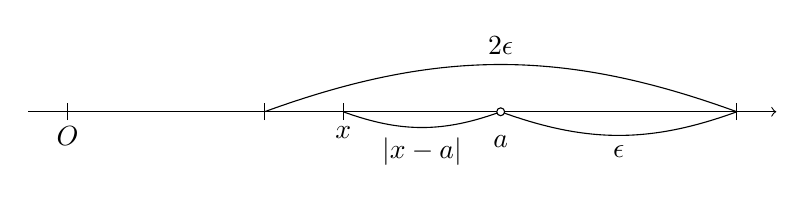
\begin{tikzpicture}
    \draw [->] (-1,0) -- (8.5,0);

    \draw (-.5,-3pt) -- (-.5,3pt) node [below=5pt] {$O$};

    \draw (2,-3pt) -- (2,3pt);
    \draw (8,-3pt) -- (8,3pt);

    \draw (2,0) to [out=20,in=160] node [above] {$2\epsilon$} (8,0);

    \draw (5,0) to [out=-20,in=-160] node [below] {$\epsilon$} (8,0);


    \draw (3,-3pt) -- (3,3pt) node [below=5pt] {$x$};

    \draw (3,0) to [out=-20,in=-160] node [below] {$|x - a|$} (5,0);

    \draw [fill=white] (5,0) circle (0.05) node [below=5pt] {$a$};
  \end{tikzpicture}

  \caption{Límite de una variable}
  \label{c:limcont:vlimdef}
\end{figure}

\begin{example}
  La variable $x$ toma valores sucesivos:

  $$x_1 = 2;\quad x_2 = 1 \frac{1}{2};\quad x_3 = 1 \frac{1}{3};\quad
  \cdots;\quad x_n = 1 \frac{1}{n};\quad \cdots$$

  Se demostrará que $\lim x = 1$. Se tiene

  $$|x_n - 1| = \left| \left(1 + \frac{1}{n}\right) - 1 \right| = \frac{1}{n}$$

  Para cualquier $\epsilon$, a partir de $n$, donde $\frac{1}{n} < \epsilon$ o $n > \frac{1}{\epsilon}$, se satisfacen la desigualdad $|x_n - 1| < \epsilon$.
\end{example}

\begin{definition} \index{límite!variable!infinito}
  Una variable $x$ se aproxima al infinito, si para cada número positivo prefijado $M$ es posible indicar un valor de $x$, de manera que todos los valores posteriores satisfacen la desigualdad $|x| > M$.
  La variable $x$ se denomina \emph{infinitamente grande}: $x \to \infty$.
\end{definition}

\begin{example}
  La variable $x$ toma los valores:
  $$x_1 = -1; \quad x_2 = 2; \quad \cdots; \quad x_n = (-1)^n n \cdots$$
\end{example}

Para $M > 0$, $x \to +\infty$ para $M < x$ o $x \to -\infty$ para $x < -M$.




%% >>> 2
\section{Límite de una función}

\begin{definition}
  La función $y = f(x)$ se aproxima al límite $b$ ($y \to b$) cuando $x \to a$, si para cada número positivo $\epsilon$ es posible indicar un número positivo $\delta$ tal que para todo $x$, diferente de $a$ y que satisface $|x - a| < \delta$, se cumple $|f(x) - b| < \epsilon$.
  $$\lim_{x \to a} f(x) = b$$
\end{definition}

Considerar que los $\epsilon$ y $\delta$ son números positivos arbitrariamente pequeños y los $N$ y $M$ son números positivos arbitrariamente grandes. % (figura \ref{c:limcont:flimdef}).

%% \begin{figure}
%%   \centering

%%   \begin{tikzpicture}
%%     \begin{axis}[ticks = none]
%%     \end{axis}
%%   \end{tikzpicture}
%%   \caption{Límite: $\epsilon$ -- $\delta$}
%%   \label{c:limcont:flimdef}
%% \end{figure}


\begin{remark}
Si \( f(x) \to b_1 \) cuando \( x \to a \), de modo que \( x < a \), el límite \emph{por la izquierda} es \( \lim_{x \to a-0} f(x) = b_1 \). Si \( x > a \) entonces el límite \emph{por la derecha} es \( \lim_{x \to a+0} f(x) = b_2 \). Si \( b_1 = b_2 = b \)  entonces \( \lim_{x \to a} f(x) = b \). Recíprocamente, si \( \lim_{x \to a} f(x) = b \) exiten los límites \( b_1 \) y \( b_2 \) que son iguales.
% imagen
\end{remark}


\begin{example}
  Para demostrar que $\lim_{x \to 2} (3x + 1) = 7$, para $|(3x + 1) - 7| < \epsilon$ se tiene

  $$|3x - 6| < \epsilon, \quad |x - 2| < \frac{\epsilon}{3}, \quad
  -\frac{\epsilon}{3} < x - 2 < \frac{\epsilon}{3}.$$

  Luego, todos los $x$ cumplen $|x - 2| < \frac{\epsilon}{3} = \delta$. Esto significa que $7$ es el límite de la función cuando $x \to 2$.
\end{example}


\begin{example}
  Para $$\lim_{x \to 2} \frac {x^2 - 4} {x - 2} = 4.$$

  $$\left| \frac {x^2 - 4} {x - 2} - 4 \right| < \epsilon$$

  $$\left| \frac {(x - 2) (x + 2)} {x - 2} - 4 \right|
  = |(x + 2) - 4| < \epsilon, \qquad |x - 2| < \epsilon$$

  Luego, se cumple la desigualdad para $\delta = \epsilon$.
\end{example}


\begin{definition}
  La función $f(x)$ se aproxima al límite $b$ cuando $x \to \infty$, si para cada $\epsilon$ es posible indicar un número positivo $N$ tal que para todos los valores de $x$ que satisfacen $|x| > N$ se cumple $|f(x) - b| < \epsilon$.
\end{definition}


\begin{example}
  Para mostrar que

  $$\lim_{x \to \infty} \left( \frac {x + 1} {x} \right) = 1$$
  o
  $$\lim_{x \to \infty} \left( 1 + \frac{1}{x} \right) = 1$$

  Es necesario demostrar que $$\left| \left( 1 + \frac{1}{x} \right) - 1 \right| < \epsilon$$ si $|x| > N$, para $N$ determinado por la elección de $\epsilon$.
  Esto se cumple cuando $|x| > \frac{1}{\epsilon} = N$ (figura \ref{c:limcont:limejnodef}).
\end{example}


\begin{figure}
  \centering

  \begin{tikzpicture}
    \begin{axis}[
        axis x line=center,
        axis y line=center,
        xlabel = $x$,
        ylabel = $y$,
        ticks = none,
        xmin=-8, xmax=19,
        ymin=-1, ymax=4,
        %% width=\textwidth
      ]

      \addplot[
        domain=-8:-.01,
        samples=100
      ]
      {(x + 1)/x};

      \addplot[
        domain=.01:19,
        samples=100
      ]
      {(x + 1)/x};

      \addplot [domain=-8:19] {1} node [pos=0.5,below=-2pt] {$y = 1$};


      \addplot [domain=-8:19, dashed] {1.5}
        node [pos=0.85,above] {$y = 1 + \epsilon$};

      \addplot [domain=-8:19, dashed] { .5}
        node [pos=0.85,above] {$y = 1 - \epsilon$};


      \addplot [black] coordinates {(.7,-.15)} node {$O$};

      \addplot [black] coordinates {(.6,.8)} node {$1$};
    \end{axis}
  \end{tikzpicture}

  \caption{$\frac{x + 1}{x}$}
  \label{c:limcont:limejnodef}
\end{figure}




%% >>> 3
\section{Función que tiende al infinito. Funciones acotadas}

\begin{definition}
  La función $f(x)$ tiende al infinito cuando $x \to a$, si para cualquier número positivo $M$ es posible hallar un $\delta > 0$ tal que para todos los valores de $x$, diferentes de $a$, y que satisfacen $|x - a| < \delta$, se tiene que $|f(x)| > M$.
  $$\lim_{x \to a} f(x) = \infty$$
\end{definition}


\begin{example}
  Para $\lim_{x \to 1} \frac {1} {(1 - x)^2} = +\infty$,

  $$\frac {1} {(1 - x)^2} > M, \quad (1 - x)^2 < \frac{1}{M}, \quad
  |1 - x| < \frac{1}{\sqrt{M}} = \delta$$
\end{example}


%% figura


\begin{example}
  Para \( \lim_{x \to 0} \left( - \frac{1}{x} \right) = \infty \).
  \[
  \left| - \frac{1}{x} > M, \right| \qquad (M > 0)
  \]
  tal que
  \[
  |x| = |x - 0| < \frac{1}{M} = \delta.
  \]
  Aquí, \( (- \frac{1}{x}) > 0 \) para \( x < 0 \) y \( (- \frac{1}{x}) < 0 \) para \( x > 0 \).
\end{example}


%% figura


Si cuando \( f(x) \) tiende al infinito cuando \( x \to \infty \), se tiene
\[ \lim_{x \to \infty} f(x) = \infty, \]
siendo los casos particulares:
\[
\lim_{x \to +\infty} f(x) =  \infty, \qquad
\lim_{x \to -\infty} f(x) =  \infty, \qquad
\lim_{x \to +\infty} f(x) = -\infty.
\]
Por ejemplo,
\[
\lim_{x \to \infty}  x^2 = +\infty, \qquad
\lim_{x \to -\infty} x^3 = -\infty.
\]


\begin{example}
  \( y = \sin x \) defini en \( -\infty < x < +\infty \), cuando \( x \to +\infty \), no tiende a ningún límite finito o infinito.
\end{example}


\begin{example} \label{ej:sen1lx}
  \( y = \sin \frac{1}{x} \) está definido para todos los valores de \( x \), excepto \( x = 0 \), no se aproxima a ningún límite finito o infinito, cuando \( x \to 0 \).
\end{example}


%% figura


\begin{definition}
  La función $y = f(x)$ está \emph{acotada} en algún intervalo de $x$ si existe un número positivo $M$ tal que $|f(x)| \le M$.
\end{definition}


\begin{definition}
  $y = f(x)$ está \emph{acotada} cuando $x \to \infty$ si existe un número $N > 0$ tal que para todos los $x$ que cumplen $|x| > N$, $f(x)$ está acotada.
\end{definition}


\begin{theorem}
  Si $\lim_{x \to a} f(x) = b$, donde $b$ es número finito, la función $f(x)$ está \emph{acotada} cuando $x \to a$.
\end{theorem}

\begin{proof}
  De $lim_{x \to a} f(x) = b$:

  $$|f(x) - b| < \epsilon$$
  $$|f(x)| < |b| + \epsilon$$

  lo que significa que $f(x)$ está acotada cuando $x \to a$.
\end{proof}


\begin{theorem} \label{sec:acotado:teo:1}
  Si $\lim_{x \to a} f(x) = b \ne 0$, entonces $y = \frac{1}{f(x)}$ está \emph{acotada} cuando $x \to a$.
\end{theorem}

\begin{proof}
  $$|f(x) - b| < \epsilon, \qquad -\epsilon < |f(x)| - |b| < \epsilon,
  \qquad |b| -\epsilon < |f(x)| < |b| + \epsilon$$
  $$\frac{1}{|b| -\epsilon} > \frac{1}{|f(x)|} > \frac{1}{|b| + \epsilon}$$
\end{proof}




%% >>> 4
\section{Infinitesimales y sus propiedades}

\begin{definition}
  La función $\alpha = \alpha(x)$ es un \emph{infinitesimal} cuando $x \to a$ o $x \to \infty$ si $\lim_{x \to a} \alpha(x) = 0$ o $\lim_{x \to \infty} \alpha(x) = 0$.
\end{definition}


\begin{theorem} \label{sec:inf:teo:suminf}
  Si $y = f(x)$ es de la forma $y = b + \alpha$, entonces $\lim y = b$ (cuando $x \to a$ o $x \to \infty$). A la inversa, si $\lim y = b$, $y = b + \alpha$, donde $b$ es una constante y $\alpha$ es un infinitesimal.
\end{theorem}

\begin{proof}
  De $y = b + \alpha$, se tiene que $|y - b| = |\alpha|$. Para un $\epsilon$ arbitrario se cumple que $|\alpha| < \epsilon$; así, $|y - b| < \epsilon$, es decir, $\lim y = b$.
  A la inversa, si $\lim y = b$, se cumple $|y - b| < \epsilon$. Si se define $y - b = \alpha$, se cumple que $|\alpha| < \epsilon$, es decir, $\alpha$ es un infinitesimal.
\end{proof}


\begin{theorem} \label{sec:inf:teo:invinf}
  Si $\alpha = \alpha(x)$ tiende a cero cuando $x \to a$ (o $x \to \infty$), sin llegar a ser cero, entonces $y = \frac{1}{\alpha}$ tiende a infinito.
\end{theorem}

\begin{proof}
  Para $M > 0$, se cumple $\frac{1}{|\alpha|} > M$ siempre que $|\alpha| < \frac{1}{M}$, lo cual es cumplido cuando $\alpha(x) \to 0$.
\end{proof}


\begin{theorem}
  La suma algebraica de un número de infinitesimales es un infinitesimal.
\end{theorem}

\begin{proof}
  La prueba para dos infinitesimales es similar para cualquier número de términos.
  Sea $u(x) = \alpha(x) + \beta(x)$, donde $\lim_{x \to a} \alpha(x) = 0$ y $\lim_{x \to a} \beta(x) = 0$.
  Como $\alpha(x)$ es un infinitesimal, se cumple $|\alpha(x)| < \frac{\epsilon}{2}$ para un $\epsilon$ arbitrario.
  De manera similar: $|\beta(x)| < \frac{\epsilon}{2}$. Entonces se tiene que
  $$|u| = |\alpha(x) + \beta(x)| \le |\alpha(x)| + |\beta(x)| < \frac{\epsilon}{2} + \frac{\epsilon}{2} = \epsilon$$
  Así, $|u| < \epsilon$, como es requerido.
  La prueba es similar cuando $\lim_{x \to \infty} \alpha(x) = 0$ y $\lim_{x \to \infty} \beta(x) = 0$.
\end{proof}


\begin{theorem} \label{sec:inf:teo:infxfunc}
  El producto de un infinitesimal $\alpha = \alpha(x)$ por una función acotada $z = z(\alpha)$, cuando $x \to a$ (o $x \to \infty)$ es un infinitesimal.
\end{theorem}

\begin{proof}
  Para $M > 0$ se cumple $|z| < M$. Para $\epsilon > 0$ se cumple $|\alpha| < \frac{\epsilon}{M}$. Luego $$|\alpha z| < \frac {\epsilon} {M} M = \epsilon$$
  es decir, $\alpha z$ es un infinitesimal. La demostración se aplica para $x \to a$ y para $x \to \infty$, de manera similar.
\end{proof}


\begin{corollary}
  Si $\lim \alpha = 0$ y $\lim \beta = 0$, entonces $\lim \alpha \beta = 0$.
  Debido a que $\beta$ es una magnitud acotada. Es válido para un número finito de factores.
\end{corollary}


\begin{corollary}
  Si $\lim \alpha = 0$ y $c = const$, entonces $\lim c\alpha = 0$.
\end{corollary}


\begin{theorem} \label{sec:inf:teo:coci}
  El cociente $\frac {\alpha(x)} {z(x)}$, donde $\alpha(x)$ es un infinitesimal y $z(x) \ne 0$, es un infinitesimal.
\end{theorem}

\begin{proof}
  Sea $\lim \alpha(x) = 0$ y $\lim z(x) = b \ne 0$. Por el Teorema \ref{sec:acotado:teo:1}, $\frac {1} {z(x)}$ es una magnitud acotada. Por eso, $\frac {\alpha(x)} {z(x)} = \alpha(x) \frac{1}{z(x)}$ es un infinitesimal.
\end{proof}




%% >>> 5
\section{Teoremas básicos del límite}


\begin{theorem}
  $\lim (u_1 + u_2 + \dots + u_k) = \lim u_1 + \lim u_2 + \dots + \lim u_k $
\end{theorem}

\begin{proof}
  El caso de dos términos se puede generalizar. Sea $\lim u_1 = a_1$ y $\lim u_2 = a_2$. Por el Teorema \ref{sec:inf:teo:suminf}
  $$u_1 = a_1 + \alpha_1, \quad u_2 = a_2 + \alpha_2$$
  En consecuencia
  $$u_1 + u_2 = (a_1 + a_2) + (\alpha_1 + \alpha_2)$$
  Como $(a_1 + a_2)$ es una constante y $(\alpha_1 + \alpha_2)$ es un infinitesimal, por el Teorema \ref{sec:inf:teo:suminf}
  $$\lim (u_1 + u_2) = a_1 + a_2 = \lim u_1 + \lim u_2$$
\end{proof}


\begin{example}
  $$\lim_{x \to \infty} \frac {x^2 + 2x} {x_2} = \lim_{x \to \infty} (1 + \frac{2}{x}) = \lim_{x \to \infty} 1 + \lim_{x \to \infty} \frac{2}{x} = 1 + \lim_{x \to \infty} \frac{2}{x} = 1 + 0 = 1$$
\end{example}


\begin{theorem}
  $\lim (u_1 \cdot u_2 \cdots u_k) = \lim u_1 \cdot \lim u_2 \cdots \lim u_k $
\end{theorem}

\begin{proof}
  Sea $\lim u_1 = a_1$ y $\lim u_2 = a_2$, entonces
  $$u_1 = a_1 + \alpha_1, \quad u_2 = a_2 + \alpha_2$$
  $$u_1 u_2 = (a_1 + \alpha_1) (a_2 + \alpha_2) = a_1 a_2 + a_1 \alpha_2 + a_2 + \alpha_1 + \alpha_1 \alpha_2$$
  $a_1 a_2$ es una constante. Por el Teorema \ref{sec:inf:teo:infxfunc}, $a_1 a_2 + a_1 \alpha_1 + a_2 \alpha_1 + \alpha_1 \alpha_2$  es un infinitesimal. Por lo tanto, $\lim u_1 u_2 = \lim u_1 \cdot \lim u_2$.
\end{proof}


\begin{corollary}
  Si $\lim u = \alpha$ y $c$ es una constante, entonces $\lim (cu) = \lim c \cdot \lim u = c \cdot \lim u$.
\end{corollary}


\begin{theorem}
  $\lim \frac {u}{v} = \frac {\lim u} {\lim v}$ si $v \ne 0$
\end{theorem}

\begin{proof}
  Sea $\lim u = a$ y $\lim v = b \ne 0$, entonces $u = a + \alpha$ y $v = b + \beta$, donde $\alpha$ y $\beta$ son infinitesimales.

  $$\frac{u}{v} = \frac {a + \alpha} {b + \beta} = \frac {a} {b} + \left( \frac {a + \alpha} {b + \beta} - \frac {a} {b} \right) = \frac {a} {b} + \frac {\alpha b - \beta a} {b (b + \beta)}$$

  $$\frac{u}{v} = \frac {a} {b} + \frac {\alpha b - \beta a} {b (b + \beta)}$$

  $\frac {a} {b}$ es una constante, mientras $\frac {a} {b} + \frac {\alpha b - \beta a} {b (b + \beta)}$ es un infinitesimal, por los Teoremas \ref{sec:inf:teo:infxfunc} y \ref{sec:inf:teo:coci}, donde $\alpha b - \beta a$ es un infinitesimal, mientras que para $b (b + \beta)$ se tiene $\lim b^2 \ne 0$. Por lo tanto, $\lim \frac{u} {v} = \frac {a} {b} = \frac {\lim u} {\lim v}$.
\end{proof}


\begin{example}
  \[ \lim_{x \to 1} \frac {3x + 5} {4x - 2} = \frac {\lim_{x \to 1} (3x + 5)} {\lim_{x \to 1} (4x - 2)} = \frac {3 \lim_{x \to 1} x + 5} {4 \lim_{x \to 1} x - 2} = \frac {3 \cdot 1 + 5} {4 \cdot 1 - 2} = \frac {8} {2} = 4\]
\end{example}


\begin{example}
  \[ \lim_{x \to 2} \frac {x^2 - 4} {x - 2} = \lim_{x \to 2} \frac {(x - 2) (x + 2)} {x - 2} = \lim_{x \to 2} (x + 2) = 4 \]
\end{example}


\begin{example}
  \[ \lim_{x \to 1} \frac {x} {x - 1} \]

  El denominador se aproxima a cero pero el numerador no. Así el límite del recíproco

  \[ \lim_{x \to 1} \frac {x - 1} {x} = \frac {\lim_{x \to 1} (x - 1)} {\lim_{x \to 1}  x} = \frac {0} {1} = 0 \]

  Por el teorema \ref{sec:inf:teo:invinf}, se tiene

  \[ \lim_{x \to 1} \frac {x} {x - 1} = \infty \]
\end{example}


\begin{theorem} \label{teo:uzvlimb}
  Si $u(x) \le z(x) \le v(x)$, donde $\lim u(x) = b$ y $\lim v(x) = b$ cuando $x \to a$ (o $x \to \infty$), entonces $\lim z(x) = b$ cuando $x \to a$ (o $x \to \infty$).
\end{theorem}

\begin{proof}
  Se tiene $u - b \le z - b \le v - b$. Como
  $$\lim_{x \to a} u(x) = b \qquad \mbox{y} \qquad \lim_{x \to a} v(x) = b$$
  se cumple
  $$-\epsilon < u - b < \epsilon \qquad \mbox{y} \qquad -\epsilon < v - b < \epsilon$$
  así
  $$-\epsilon < z - b < \epsilon$$
  es decir
  $$\lim_{x \to a} z = b$$
\end{proof}


\begin{theorem} \label{sec:blim:teo:bMo}
  Si cuando $x \to a$ (o $x \to \infty$) la función $y \ge 0$ y $\lim y = b$, entonces $b \ge 0$.
\end{theorem}

\begin{proof}
  Asumiendo \( b < 0 \), entonces \( |y - b| \ge b \), así, \( \neg (y \to b) \) cuando \( x \to a \), lo que contradice la afirmación. Por lo tanto, \( b < 0 \) lleva a una contradicción. Consecuentemente, \( b \ge 0 \).
\end{proof}


\begin{theorem} \label{teo:limvMlimu}
  Si $v \ge u$ se cumple las funciones $u = u(x)$ y $v = v(x)$, que se aproximan a algún límite cuando $x \to a$ (o $x \to \infty$), entonces $\lim v \ge \lim u$.
\end{theorem}

\begin{proof}
  Dado \( v - u \ge 0 \). Por lo tanto, por el Teorema \ref{sec:blim:teo:bMo}, \( \lim (v - u) \ge 0 \) o \( \lim v - \lim u \ge 0 \), así, \( \lim v \ge \lim u \).
\end{proof}


\begin{example}
  \[ \lim_{x \to 0} \sin x = 0 \]

  De la Figura \ref{fig:sintoo}, si \( OA = 1 \), entonces \( AC = \sin x \), \( \wideparen{AB} = x \) y \( \sin x < x \) (\( |\sin x| < |x| \)). Por los Teoremas \ref{sec:blim:teo:bMo} y \ref{teo:limvMlimu}, \( \lim_{x \to 0} \sin x = 0 \).
\end{example}


\begin{example} \label{ej:sinxl2}
  \[ \lim_{x \to 0} \sin \frac{x}{2} = 0\]
  En consencuencia a \( \left| \sin \frac{x}{2} \right| < |\sin x| \).
\end{example}


\begin{example}
  \[ \lim_{x \to 0} \cos x = 1 \]
  Considerando
  \[ \cos x = 1 - 2 \sin^2 \frac{x}{2} \]
  entonces
  \[ \lim_{x \to 0} \cos x = \lim_{x \to 0} \left( 1 - 2 \sin^2 \frac{x}{2} \right) = 1 - 2 \lim_{x \to 0} \sin^2 \frac{x}{2} = 1 - 0 = 1\]
\end{example}


\begin{figure}
  \centering

  \begin{tikzpicture}
    \begin{axis}[
        axis x line=center,
        axis y line=center,
        axis line style={-},
        ticks = none,
        %% xmin=-8, xmax=19,
        %% ymin=-1, ymax=4,
        %% width=\textwidth
      ]

      \addplot[
        domain=0:1,
        samples=110
      ]
      {(1 - x^2)^(1/2)};


      \addplot[
        domain=0:.82,
        samples=110
      ]
      { .7 * x};


      \draw ({rel axis cs:0,0} -| {axis cs:.819,0}) -- ({rel axis cs:0,.574} -| {axis cs:.819,0});

      \draw ({rel axis cs:0,0} -| {axis cs:1,0}) -- ({rel axis cs:0,.574} -| {axis cs:.819,0});


      \addplot [black] coordinates {(.849,.604)} node {$A$};

      \addplot [black] coordinates {(.849,.04)} node {$C$};

      \addplot [black] coordinates {(.95,.04)} node {$B$};

      \addplot [black] coordinates {(.1,.035)} node {$O$};

      %% \addplot [black] coordinates {(.7,-.15)} node {$O$};

      %% \addplot [black] coordinates {(.6,.8)} node {$1$};
    \end{axis}
  \end{tikzpicture}

  \caption{Semi-circunferencia \( \sin x \)}
  \label{fig:sintoo}
\end{figure}


\begin{theorem} \label{teo:limcreacot}
  Si $v$ es creciente ($v_i \le v_{i+1}$) y acotada ($v < M$), entonces $\lim v = a$, donde $a \le M$.
\end{theorem}

%% \begin{proof}

%% \end{proof}




%% >>> 6
\section{Límite de la función $\frac {\sin x} {x}$ cuando $x \to 0$}

De la figura \ref{fig:sintoo}, el \( \sin x \) es menor que el arco \( x \), que a su vez es menor que \( \tan x \), es decir

\[ \sin x < x < \tan x \]
\[ 1 < \frac {x} {\sin x} < \frac {1} {\cos x} \]
\[ 1 > \frac {\sin x} {x} > \cos x \]

Luego, como \( \lim_{x \to 0} 1 = 1 \) y \( \lim_{x \to 0} \cos x = 1 \), por el eorema \ref{teo:uzvlimb},

\[ \lim_{x \to 0} \frac {\sin x} {x} = 1 \]


\begin{example}
  \[ \lim_{x \to 0} \frac {\tan x} {x} = \lim_{x \to 0}  \frac {\sin x} {x} \cdot \frac {1} {\cos x} = \lim_{x \to 0} \frac {\sin x} {x} \cdot \lim_{x \to 0} \frac {1} {\cos x} = 1 \cdot \frac{1}{1} = 1\]
\end{example}


\begin{example}
  \[ \lim_{x \to 0} \frac {\sin kx} {x} = \lim_{x \to 0} k \frac {\sin kx} {kx} = k \lim_{\begin{array}{c}x \to 0 \\ (kx \to 0)\end{array}} \frac {\sin(kx)} {(kx)} = k \cdot 1 = k \qquad(k = const)\]
\end{example}


\begin{example}
  \[ \lim_{x \to 0} \frac {1 - \cos x} {x} = \lim_{x \to 0} \frac{2\sin^2\frac{x}{2}} {x} = \lim_{x \to 0} \frac{\sin\frac{x}{2}} {\frac{x}{2}} \sin \frac{x}{2} = 1 \cdot 0 = 0 \]
\end{example}


\begin{example}
  \[ (\alpha = const, \quad \beta = const) \]
  \[ \lim_{x \to 0} \frac {\sin \alpha x} {\sin \beta x} = \lim_{x \to 0} \frac {\alpha} {\beta} \cdot \frac {\frac{\sin \alpha x}{\alpha x}} {\frac {\sin \beta x} {\beta x}} = \frac {\alpha} {\beta} \frac {\lim_{x \to 0}  \frac {\sin \alpha x} {\alpha x}} {\lim_{x \to 0} \frac {\sin \beta x} {\beta x}} = \frac {\alpha} {\beta} \cdot \frac {1} {1} = \frac {\alpha} {\beta} \]
\end{example}




%% >>> 7
\section{El número $e$}

\begin{theorem}
  La variable \( (1 + \frac{1}{n})^n \), cuando \( x \to \infty \), tiene un límite entre \(2\) y \(3\).
\end{theorem}

\begin{proof}
  Por el Binomio de Newton
  \begin{align} \label{eq:binomlime}
    \begin{split}
      \left( 1 + \frac{1}{n} \right)^n & = 1
      + \frac{n}{1} \frac{1}{n}
      + \frac{n(n - 1)}{1 \cdot 2} \cdot \left( \frac{1}{n} \right)^2
      + \frac{n(n - 1)(n - 2)}{1 \cdot 2 \cdot 3} \left( \frac{1}{n} \right)^3
      + \cdots
      \\ & \qquad
      \cdots
      + \frac{n(n - 1)(n - 2) \cdots [n - (n - 1)]}
             {1 \cdot 2 \cdot \ldots \cdot n} \left( \frac{1}{n} \right)^n
      \\\\
      & = 1
      + 1
      + \frac{1}{1 \cdot 2} \left( 1 - \frac{1}{n} \right)
      + \frac{1}{1 \cdot 2 \cdot 2}
        \left( 1 - \frac{1}{n} \right)
        \left( 1 - \frac{2}{n} \right)
      + \cdots
      \\ & \qquad
      \cdots
      + \frac{1}{1 \cdot 2 \cdot \ldots \cdot n}
        \left( 1 - \frac{1}{n} \right)
        \left( 1 - \frac{2}{n} \right)
        \cdots
        \left( 1 - \frac{n - 1}{n} \right)
    \end{split}
  \end{align}

  De la igualdad, \( \left( 1 + \frac{1}{n} \right)^n \) es creciente. Así, incrementa de \(n\) a \(n + 1\):
  \[ \frac{1}{1 \cdot 2} \left( 1 - \frac{1}{n} \right) < \frac{1}{1 \cdot 2} \left( 1 - \frac{1}{n + 1} \right) \]

  y de manera similar para los otros términos. Para mostrar que \( \left( 1 + \frac{1}{n} \right)^n \) es acotada, se aprecia que
  \[ \left( 1 - \frac{1}{n} \right) < 1, \quad \left( 1 - \frac{1}{n} \right) \left( 1 - \frac{2}{n} \right) < 1 \]

  etc., de la expresión \ref{eq:binomlime} se obtiene la igualdad
  \[ \left( 1 + \frac{1}{n} \right)^n < 1 + 1 + \frac{1}{1 \cdot 2} + \frac{1}{1 \cdot 2 \cdot 3} + \cdots + \frac{1}{1 \cdot 2 \cdot 3 \cdot \ldots \cdot n} \]

  Además considerando que
  \[ \frac{1}{1 \cdot 2 \cdot 3} < \frac{1}{2^2}; \qquad
     \frac{1}{1 \cdot 2 \cdot 3 \cdot 4} < \frac{1}{2^3}; \qquad
     \frac{1}{1 \cdot 2 \cdot \ldots \cdot n} < \frac{1}{2^{n - 1}} \]

  Se puede escribir la desigualdad
  \begin{align*}
     \left( 1 + \frac{1}{n} \right)^n & < 1 + 1 + \frac{1}{2} + \frac{1}{2^2} + \cdots + \frac{1}{2^{n -1}}
     \\ &
     < 1 + \left( 1 + \frac{1}{2} + \frac{1}{2^2} + \cdots + \frac{1}{2^{n -1}} \right)
  \end{align*}

  Los términos agrupados forman una progresión geométrica siendo la razón \( q = \frac{1}{2} \) y el primer término \( a = 1 \), así

  \[ \frac{1}{1 \cdot 2 \cdot 3} < 1 + \left[ 1 + \frac{1}{2} + \frac{1}{2^2} + \cdots + \frac{1}{2^{n -1}} \right] = \]
  \[ = 1 + \frac{a - aq^n}{1 - q} = 1 + \frac{1 - \left(\frac{1}{2}\right)^2}{1 - \frac{1}{2}} = 1 + \left[ 2 - \left(\frac{1}{2}\right)^{n - 1} \right] < 3 \]

  De la igualdad \ref{eq:binomlime} se sigue

  \[ \left( 1 + \frac{1}{n} \right)^n \ge 2 \]

  Por lo tanto,

  \begin{equation} \label{eq:limeacotinter}
    2 \le \left( 1 + \frac{1}{n} \right)^n < 3
  \end{equation}
\end{proof}


Esto prueba que \( \left( 1 + \frac{1}{n} \right)^n \) está acotada. Así, al ser creciente y acotada, por el Teorema \ref{teo:limcreacot}, este tiene un límite, que es denotado por \(e\).


\begin{definition}
  El límite de la variable \( \left( 1 + \frac{1}{n} \right)^n \) cuando \( n \to \infty \) es el número \( e \):
  \[ e = \lim_{n \to \infty} \left( 1 + \frac{1}{n} \right)^n \]
\end{definition}


Por el Teorema \ref{teo:limvMlimu}, se sigue de la desigualdad \ref{eq:limeacotinter} que se satisface \( 2 \le e \le 3 \).


\begin{theorem}
  La función \( \left( 1 + \frac{1}{x} \right)^x \) tiende al límite \(e\) cuando \(x\) tiende al infinito, \( \lim_{x \to \infty} \left( 1 + \frac{1}{x} \right)^x = e \).
\end{theorem}


\begin{proof}
  Se ha probado que \( \left( 1 + \frac{1}{n} \right)^n \to e \) cuando \( x \to \infty \), si \(n\) toma valores enteros positivos. Ahora \(x\) tiende al infinito tomando valores fracionarios y negativos.

  1) Sea \( x \to +\infty \), cada uno de sus valores se encuntra entre dos números enteros positivos.
  \[ n \le x < n + 1 \]
  Se cumplen
  \[ \frac{1}{n} \ge \frac{1}{x} > \frac{1}{n + 1} \]
  \[ 1 + \frac{1}{x} \ge 1 + \frac{1}{x} > 1 + \frac{1}{n + 1} \]
  \[ \left( 1 + \frac{1}{x} \right)^{n + 1} \ge \left( 1 + \frac{1}{x} \right)^{x} > \left( 1 + \frac{1}{n + 1} \right)^{n} \]
  Si \( x \to \infty \) es obvio que \( n \to \infty \). Hallando lo límites de las variables entre las cuales \( \left( 1 + \frac{1}{x} \right)^x \) se encuentra:
  \begin{align*}
    \lim_{n \to +\infty} \left( 1 + \frac{1}{n} \right)^{n + 1} & =
    \lim_{n \to +\infty} \left( 1 + \frac{1}{n} \right)^n
      \left( 1 + \frac{1}{n} \right) =
    \\ & =
    \lim_{n \to +\infty} \left( 1 + \frac{1}{n} \right)^n \cdot
      \lim_{n \to +\infty} \left( 1 + \frac{1}{n} \right)
    = e \cdot 1 = e
    \\
    \\
    \lim_{n \to +\infty} \left( 1 + \frac{1}{n + 1} \right)^{n} & =
    \lim_{n \to +\infty}
      \frac {\left( 1 + \frac{1}{n + 1} \right)^{n + 1}}
            {1 + \frac{1}{n + 1}} =
    \\ & =
    \frac {\lim_{n \to +\infty} \left( 1 + \frac{1}{n + 1} \right)^{n + 1}}
          {\lim_{n \to +\infty} \left( 1 + \frac{1}{n + 1} \right) }
    = \frac{e}{1} = e
  \end{align*}
  Por lo tanto, por el Teorema \ref{teo:uzvlimb},
  \[ \lim_{x \to +\infty} \left( 1 + \frac{1}{x} \right)^x = e \]

  2) Sea \( x \to -\infty \), si se define \( t = - (x + 1) \) o \( x = -(t + 1) \), cuando \( t \to +\infty \) entonces \( x \to -\infty \).
  \begin{align*}
   \lim_{x \to -\infty} \left( 1 + \frac{1}{x} \right)^x & = \lim_{t \to +\infty} \left( 1 - \frac{1}{t + 1} \right)^{-t-1} = \lim_{t \to +\infty} \left( \frac{t}{t + 1} \right)^{-t-1} = \\
   & = \lim_{t \to +\infty} \left( \frac{t + 1}{t} \right)^{t + 1} = \lim_{t \to +\infty} \left( 1 + \frac{1}{t} \right)^{t + 1} = \\
   & = \lim_{t \to +\infty} \left( 1 + \frac{1}{t} \right)^t \left( 1 + \frac{1}{t} \right) = e \cdot 1 = e
  \end{align*}
\end{proof}


%\begin{figure}
%  %% y = (1 + 1/x) ^x
%\end{figure}


Usando \( \frac{1}{x} = \alpha \), cuando \( x \to \infty \) se tiene \( \alpha \to 0 \) (\( \alpha \ne 0 \)).
\[ \lim_{\alpha \to 0} (1 + \alpha)^{\frac{1}{\alpha}} \]


\begin{example}
  \begin{align*}
    \lim_{n \to \infty} \left( 1 + \frac{1}{n} \right)^{n + 5}
    & = \lim_{n \to \infty}
      \left( 1 + \frac{1}{n} \right)^n
      \left( 1 + \frac{1}{n} \right)^5 =
    \\ & =
    \lim_{n \to \infty} \left( 1 + \frac{1}{n} \right)^n
    \cdot \lim_{n \to \infty} \left( 1 + \frac{1}{n} \right)^5
    = e \cdot 1 = e
  \end{align*}
\end{example}


\begin{example}
  \[
    \lim_{x \to \infty} \left( 1 + \frac{1}{x} \right)^{3x}
    = \lim_{x \to \infty} \left( 1 + \frac{1}{x} \right)^x
                          \left( 1 + \frac{1}{x} \right)^x
                          \left( 1 + \frac{1}{x} \right)^x =
  \]
  \[
    = \lim_{x \to \infty} \left( 1 + \frac{1}{x} \right)^x \cdot
      \lim_{x \to \infty} \left( 1 + \frac{1}{x} \right)^x \cdot
      \lim_{x \to \infty} \left( 1 + \frac{1}{x} \right)^x
    = e \cdot e \cdot e = e^3
  \]
\end{example}


\begin{example}
  \[ \lim_{x \to \infty} \left( 1 + \frac{2}{x} \right)^x = \lim_{y \to \infty} \left( 1 + \frac{1}{y} \right)^{2y} = e^2 \]
\end{example}


\begin{example}
  \begin{align*}
    \lim_{x \to \infty} \left( \frac{x + 3}{x - 1} \right)^{x + 3} &
    = \lim_{x \to \infty} \left( \frac{x - 1 + 4}{x - 1} \right)^{x + 3}
    = \lim_{x \to \infty} \left( 1 + \frac{4}{x - 1} \right)^{x + 3} =
    \\ &
    = \lim_{x \to \infty} \left( 1 + \frac{4}{x - 1} \right)^{(x - 1) + 4}
    = \lim_{y \to \infty} \left( 1 + \frac{4}{y} \right)^{y + 4} =
    \\ &
    = \lim_{y \to \infty} \left( 1 + \frac{4}{y} \right)^{y}
      \cdot \lim_{y \to \infty} \left( 1 + \frac{4}{y} \right)^{4}
    = e^4 \cdot 1 = e^4
  \end{align*}
\end{example}




%% >>> 8
\section{Logaritmos naturales}

\[ \log x = \frac{1}{\ln 10} \ln x \]


%% >>> 9
\section{Continuidad de las funciones}

% \begin{figure} continuidad
% \end{figure}

\begin{definition}
  La función \( y = f(x) \) es \emph{continua} para el valor \( x = x_0 \) si
  \begin{equation} \label{eq:condicioncontinuidad}
  \lim_{\Delta x \to 0} \left[ f(x_0 + \Delta x) - f(x_0) \right] = 0
  \end{equation}
  \[
  \text{o} \qquad
  \lim_{\Delta x \to 0} \Delta y = 0
  \]
\end{definition}


\begin{example}
  Mostrar que \( y = x^2 \) es continua en un punto arbitrario \( x_0 \).
  \[
  y_0 = x_0^2, \quad
  y_0 + \Delta y = \left( x_0 + \Delta x \right)^2, \quad
  \Delta y = \left( x_0 + \Delta x \right)^2 - x_0^2
  = 2 x_0 \Delta x + \Delta x^2
  \]
  \[
  \lim_{\Delta x \to 0} \Delta y
  = \lim_{\Delta x \to 0} \left( 2 x_0 \Delta x + \Delta x^2 \right)
  = 2x \lim_{\Delta x \to 0} \Delta x
    + \lim_{\Delta x \to 0} \Delta x \cdot \lim_{\Delta x \to 0} \Delta x = 0
  \]
\end{example}


% \begin{figure} parábola continudad ejemplo
% \end{figure}


\begin{example}
  Mostrar que \( y = \sin x \) es continua en un punto arbitrario \( x_0 \).
  \[
  y_0 = \sin x_0, \quad
  y_0 + \Delta y = \sin \left( x_0 + \Delta x \right),
  \]
  \[
  \Delta y = \sin \left( x_0 + \Delta x \right) - \sin x_0
  = 2 \sin \frac {\Delta x} {2}
    \cdot \cos \left( x_0 + \frac {\Delta x} {2} \right)
  \]
  Como se mostró en el ejemplo \ref{ej:sinxl2}, \( \lim_{\Delta x \to 0} \sin \frac {\Delta x} {2} = 0 \). La función \( \cos ( x + \frac {\Delta x} {2} ) \) es acotada. Por lo tanto, \( \lim_{\Delta x \to 0} \Delta y = 0 \).
\end{example}


\begin{theorem}
  Toda función elemental es continua en cada punto en la que está definida.
\end{theorem}


La condición de continuidad \ref{eq:condicioncontinuidad} pude ser escrita como
\[ \lim_{\Delta x \to 0} f(x_0 + \Delta x) = f(x_0) \]
o
\[ \lim_{x \to x_0} f(x) = f(x_0) \text{,} \]
además
\[ x_0 = \lim_{x \to x_0} x \text{,} \]
consecuentemente,
\[ \lim_{x \to x_0} f(x) = f \left( \lim_{x \to x_0} x \right) \text{.} \]
En otras palabras, para hallar el límite en una función continua, cuando \( x \to x_0 \), basta con sustituir en la expresión de la función es valor del argumento \( x_0 \), en lugar de \( x \).


\begin{example}
  \( y = x^2 \) es continua en todo punto \( x_0 \), entonces
  \[ \lim_{x \to x_0} x^2 = x_0^2 \text{,} \]
  \[ \lim_{x \to 3} x^2 = 3^2 = 9\text{.} \]
\end{example}


\begin{example}
  \( y = \sin x \) es continua en todo punto \( x_0 \), entonces
  \[
  \lim_{x \to \frac{\pi}{4}} \sin x = \sin \frac{\pi}{4} = \frac {\sqrt{2}} {2}
  \text{.}
  \]
\end{example}


\begin{example}
  \( y = e^x \) es continua en todo punto, entonces \( \lim_{x \to a} e^x = e^aa \).
\end{example}


\begin{example} \label{ej:ln1yxlx}
  \[
  \lim_{x \to 0} \frac {\ln \left( 1 + x \right)} {x}
  = \lim_{x \to 0} \frac{1}{x} \ln \left( 1 + x \right)
  = \lim_{x \to 0} \ln \left[ \left( 1 + x \right) ^{\frac{1}{x}} \right]
  \text{.}
  \]
  Como \( \lim_{x \to 0} \left( 1 + x \right) ^{\frac{1}{x}} = e \) y la función \( \ln z \) es continua para \( z > 0 \), por consiguiente, para \( z = e \),
  \[
  \lim_{x \to 0} \ln \left[ \left( 1 + x \right) ^{\frac{1}{x}} \right]
  = \ln \left[ \lim_{x \to 0} \left( 1 + x \right) ^{\frac{1}{x}} \right]
  = \ln e = 1 \text{.}
  \]
\end{example}


\begin{definition}
  Si \( y = f(x) \) es continua en cada punto del intervalo \( (a, b) \), donde \( a < b \), entonces la función \emph{es continua en ese intervalo}.
\end{definition}


Si \( \lim_{x \to a + 0} f(x) = f(a) \), \( f(x) \) en el punto \( x = a \) es \emph{continua por la derecha}. De manera similar para \( \lim_{x \to b - 0} f(x) = f(a) \).
Si \( f(x) \) es continua en cada punto del intervalo \( (a, b) \) y es continua en los puntos extremos, entonces \( f(x) \) \emph{es continua en el intervalo cerrado} \( [a, b] \).

Si en el punto \( x = x_0 \), al menos una de las condiciones no es cumplida para \( f(x) \), es decir, if para \( x = x_0 \) la función no está definida o no existe el límite \( \lim_{x \to x_0} f(x) \) o \( \lim_{x \to x_0} f(x) \ne f(x_0) \), aun cuando los límites extremos existen, entonces en el punto \( x = x_0 \) la función es \emph{discontinua}.


\begin{example}
  \( y = \frac{1}{x} \) es discontinua en \( x = 0 \). \( y \) no está definida en \( x = 0 \).
  \[
  \lim_{x \to 0+0} \frac{1}{x} = +\infty; \qquad
  \lim_{x \to 0-0} \frac{1}{x} = -\infty
  \]
  Es fácil mostrar qué es continua para cualquier \( x \ne 0 \).
\end{example}


\begin{example}
  \( y = 2^{\frac{1}{x}} \) es discontinua en \( x = 0 \).
  \[
  \lim_{x \to 0+0} 2^{\frac{1}{x}} = \infty; \qquad
  \lim_{x \to 0-0} 2^{\frac{1}{x}} = 0
  \]
  La función no está definida en \( x = 0 \).
\end{example}


%% figura para ejemplo previo y siguiente


\begin{example} \label{ex:discont}
  \( f(x) = \frac {x} {|x|} \). En \( x < 0 \), \( \frac{x}{|x|} = -1 \); en \( x > 0 \), \( \frac{x}{|x|} = 1 \). Por eso,
  \[
  \lim_{x \to 0-0} f(x) = \lim_{x \to 0-0} \frac{x}{|x|} = -1 \text{;}
  \]
  \[
  \lim_{x \to 0+0} f(x) = \lim_{x \to 0+0} \frac{x}{|x|} = 1 \text{;}
  \]
  la  función no está definida en \( x = 0 \). Así, \( f(x) = \frac{x}{|x|} \) es discontinua en \( x = 0 \).
\end{example}


\begin{example}
  \( y = \sin \frac{1}{x} \) es discontinua en \( x = 0 \).
\end{example}


\begin{definition}
  Si para la función \( f(x) \) existen los límites finitos \( \lim_{x \to x_0+0} = f(x_0 + 0) \) y \( \lim_{x \to x_0-0} = f(x_0 - 0) \). Pero, si \( \lim_{x \to x_0+0} \ne \lim_{x \to x_0-0} \) o el valor de \( f(x) \) en \( x = x_0 \) no está definida, entonces \( x = x_0 \) es el \emph{punto de discontinuidad de primer género}.
\end{definition}

Por ejemplo en el Ejemplo \ref{ex:discont}, el punto \( x = 0 \) es un punto de discontinuidad de primer género.




%% >>> 10
\section{Algunas propiedades de las funciones continuas}

\begin{theorem}
  Si \( y = f(x) \) es continua en el \( [a, b] \) (\( a \le x \le b \)), entonces en este intervalo existe al menos:
  \begin{description}
  \item un punto \( x = x_1 \) tal que \( f(x_1) \ge f(x) \) y
  \item un punto \( x = x_2 \) tal que \( f(x_2) \le f(x) \),
  \end{description}
  donde
  \begin{description}
  \item \( f(x_1) \) es el \emph{valor máximo} y
  \item \( f(x_2) \) es el \emph{valor mínimo}.
  \end{description}
\end{theorem}


%% figura


\begin{remark}
  La función podría no ser continua en \( a < x < b \). Por ejemplo, \( y = x \) en el intervalo \( 0 < x < 1 \).
\end{remark}


\begin{theorem}
  Si la función \( y = f(x) \) es continua en el intervalo \( [a, b] \) y los puntos extremos toman valores de signos contrarios, entonces existe al menos un punto \( x = c \) que cumple
  \[ f(c) = 0, \qquad a < c < b. \]
\end{theorem}


%% figura


\begin{theorem}
  Sea \( y = f(x) \) es definida y continua en \( [a, b] \). Si \( f(a) = A \) y \( f(b) = B \), entonces para \( \mu \) entre \( A \) y \( B \), habrá un punto \( x = c \) entre \( a \) y \( b \) tal que \( f(c) = \mu \).
\end{theorem}


%% figura


\begin{corollary}
  Si \( y = f(x) \) es continua en un intervalo y toma un valor máximo y mínimo, entonces habrá al menos un valor entre los vaores mínimo y maximo.
\end{corollary}


%% figura




\section{Comparación de infinitesimales}

\begin{definition}
 Si \( \lim \frac {\beta} {\alpha} = A \ne 0\) y \( \lim \frac {\alpha} {\beta} = \frac {1} {A} \ne 0 \), \( \alpha \) y \( \beta \) son \emph{infinitesimales del mismo orden}.
\end{definition}


\begin{example}
  \( \alpha = x \), \( \beta = \sin 2x \), donde \( x \to 0 \), \( \alpha \) y \( \beta \) son infinitesimales del mismo orden.
  \[
  \lim_{x \to 0} \frac{\beta}{\alpha} = \lim_{x \to 0} \frac{\sin 2x}{x} = 2.
  \]
\end{example}


\begin{example}
  Cuando \( x \to 0 \), los infinitesimales \( x \), \( \sin 3x \), \( \tan 2x \), \( 7 \ln (1 + x) \) son infinitesimales del mismo orden.
\end{example}


\begin{definition}
  Si \( \lim \frac{\beta}{\alpha} = 0 \) (y \( \lim \frac{\alpha}{\beta} = \infty \), entonces \( \beta \) es un \emph{infinitesimal de orden superior que} \( \alpha \) o \( \alpha \) es un \emph{infinitesimal de orden inferior que} \( \beta \).
\end{definition}


\begin{example}
  Sea \( \alpha = x \), \( \beta = x^n \), \( n > 1 \), \( x \to 0 \). \( \beta \) es un infinitesimal de orden superior que \( \alpha \), debido a
  \[
  \lim_{x \to 0} \frac{x^n}{x} = \lim_{x \to 0} x^{n - 1} = 0.
  \]
\end{example}


\begin{definition}
  \( \beta \) es \emph{un infinitesimal de orden \( k \) respecto a} \( \alpha \), si \( \beta \) y \( \alpha^k \) son infinitesimales del mismo orden, esto es, \( \lim \frac{\beta}{\alpha^k} = A \ne 0 \).
\end{definition}


\begin{example}
  Si \( \alpha = x \), \( \beta = x^3 \), entonces, cuando \( x \to 0 \), \( \beta \) es un infinitesimal de tercer orden respecto a \( \alpha \), dado que
  \[
  \lim_{x \to 0} \frac{\beta}{\alpha^3} = \lim_{x \to 0} \frac{x^3}{(x)^3} = 1.
  \]
\end{example}


\begin{definition}
  Si \( \lim \frac{\beta}{\alpha} = 1 \), \( \beta \) y \( \alpha \) son \emph{infinitesimales equivalentes}, \( \alpha \approx \beta \)
\end{definition}


\begin{example}
  Sea \( \alpha = x \) y \( \beta = \sin x \), cuando \( x \to 0 \). \( \alpha \) y \( \beta \) son equivalentes, debido a
  \[
  \lim_{x \to 0} \frac{\sin x}{x} = 1.
  \]
\end{example}


\begin{example}
  Sea \( \alpha = x \) y \( \beta = \ln (1 + x) \), cuando \( x \to 0 \). \( \alpha \) y \( \beta \) son equivalentes, debido a
  \[
  \lim_{x \to 0} \frac{\ln (1 + x)}{x} = 1
  \]
  (ver Ejemplo \ref{ej:ln1yxlx}).
\end{example}


\begin{theorem}
  Si \( \alpha \) y \( \beta \) sin infinitesimales equivalentes, su diferencia \( \alpha - \beta \) es un infinitesimal de orden superior que \( \alpha \) y que \( \beta \).
\end{theorem}

\begin{proof}
  \[
  \lim \frac{\alpha - \beta}{\alpha} = \lim \left( 1 - \frac{\beta}{\alpha} \right) = 1 - \lim \frac{\beta}{\alpha} = 1 - 1 = 0.
  \]
\end{proof}


\begin{theorem}
  Si \( \alpha - \beta \) es un infinitesimal de orden superior que \( \alpha \) y que \( \beta \), entonces \( \alpha \) y \( \beta \) sin infinitesimales equivalentes.
\end{theorem}

\begin{proof}
  Si \( \lim \frac{\alpha - \beta}{\alpha} = 0 \), entonces \( \lim \left( 1 - \frac{\beta}{\alpha} \right) \), o \( 1 - \lim \frac{\beta}{\alpha} = 0 \), o \( 1 = \lim \frac{\beta}{\alpha} \), es decir, \( \alpha \approx \beta \). Si \( \lim \frac{\alpha - \beta}{\beta} = 0 \), entonces \( \lim \left( \frac{\alpha}{\beta} - 1 \right) = 0 \), \( \lim \frac{\alpha}{\beta} = 1 \), esto es, \( \alpha \approx \beta \).
\end{proof}


\begin{example}
  Sea \( \alpha = x \), \( \beta = x + x^3 \), donde \( x \to 0 \). Entonces, \( \beta - \alpha = x^3 \) es un infinitesimal de orden superior que \( \alpha \) y que \( \beta \).
  \[
  \lim_{x \to 0} = \frac{\beta - \alpha}{\alpha} = \lim_{x \to 0} = \frac{x^3}{x} = \lim_{x \to 0} x^2 = 0,
  \]
  \[
  \lim_{x \to 0} = \frac{\beta - \alpha}{\beta} = \lim_{x \to 0} = \frac{x^3}{x + x^3} = \lim_{x \to 0} \frac{x^2}{1 + x^2} = 0.
  \]
\end{example}


\begin{example}
  Cuando \( x \to \infty \), \( \alpha = \frac{x + 1}{x^2} \) y \( \beta = \frac{1}{x} \) son equivalentes, ya que su diferencia \( \alpha - \beta = \frac{x + 1}{x^2} - \frac{1}{x} = \frac{1}{x^2}\) es un infinitesimal de orden superior que \( \alpha \) y que \( \beta \). El límite de la razón de \( \alpha \) y \( \beta \) es la unidad:
  \[
  \lim \frac{\beta}{\alpha} = \lim_{x \to \infty} \frac{\frac{1}{x}}{\frac{x + 1}{x^2}} = \lim_{x \to \infty} \frac{x + 1}{x} = \lim_{x \to \infty} \left( 1 + \frac{1}{x} \right) = 1.
  \]
\end{example}


\begin{remark}
  Si \( \frac{\beta}{\alpha} \) no tiene límite y no se aproxima al infinito, entonces \( \beta \) y \( \alpha \) no son comparables en el sentido anterior.
\end{remark}


\begin{example}
  Sea \( \alpha = x \), \( \beta = x \sin \frac{1}{x} \), donde \( x \to 0 \). \( \alpha \) y \( \beta \) no pueden ser comparados porque \( \frac{\beta}{\alpha} = \sin \frac{1}{x} \), cuando \( x \to 0 \), no se aproxima a un límite finito ni infinito (ver Ejemplo \ref{ej:sen1lx}).
\end{example}




%% >>>
\section*{Ejercicios}

\begin{exercise}
  \[
  \lim_{x \to 1} \frac{x^2 + 2x + 5}{x^2 + 1}.
  \qquad \text{R.} \, 4.
  \]
\end{exercise}


\begin{exercise}
  \[
  \lim_{x \to \frac{\pi}{2}} [ 2\sin x - \cos x + \cot x].
  \qquad \text{R.} \, 2.
  \]
\end{exercise}


\begin{exercise}
  \[
  \lim_{x \to 2} \frac{x - 2}{\sqrt{2 + x}}.
  \qquad \text{R.} \, 0.
  \]
\end{exercise}
























%% >>>
